\documentclass[c]{beamer}  % [t], [c], или [b] --- вертикальное выравнивание на слайдах (верх, центр, низ)

%\documentclass[handout]{beamer} % Раздаточный материал (на слайдах всё сразу)
%\documentclass[aspectratio=169]{beamer} % Соотношение сторон

%\usetheme{Berkeley} % Тема оформления
%\usetheme{Bergen}
%\usetheme{Szeged}

%\usecolortheme{beaver} % Цветовая схема
%\useinnertheme{circles}
%\useinnertheme{rectangles}

%%% Работа с русским языком
\usepackage{cmap}					% поиск в PDF
\usepackage{mathtext} 				% русские буквы в формулах
\usepackage[T2A]{fontenc}			% кодировка
\usepackage[utf8]{inputenc}			% кодировка исходного текста
\usepackage[english,russian]{babel}	% локализация и переносы

%% Beamer по-русски
\newtheorem{rtheorem}{Теорема}
\newtheorem{rproof}{Доказательство}
\newtheorem{rexample}{Пример}

%%% Дополнительная работа с математикой
\usepackage{amsmath,amsfonts,amssymb,amsthm,mathtools} % AMS
\usepackage{icomma} % "Умная" запятая: $0,2$ --- число, $0, 2$ --- перечисление

%% Номера формул
\mathtoolsset{showonlyrefs=true} % Показывать номера только у тех формул, на которые есть \eqref{} в тексте.
%\usepackage{leqno} % Нумерация формул слева

%% Свои команды
\DeclareMathOperator{\sgn}{\mathop{sgn}}

%% Перенос знаков в формулах (по Львовскому)
\newcommand*{\hm}[1]{#1\nobreak\discretionary{}
{\hbox{$\mathsurround=0pt #1$}}{}}

%%% Работа с картинками
\usepackage{graphicx}  % Для вставки рисунков
\graphicspath{{images/}{images2/}}  % папки с картинками
\setlength\fboxsep{3pt} % Отступ рамки \fbox{} от рисунка
\setlength\fboxrule{1pt} % Толщина линий рамки \fbox{}
\usepackage{wrapfig} % Обтекание рисунков текстом

%%% Работа с таблицами
\usepackage{array,tabularx,tabulary,booktabs} % Дополнительная работа с таблицами
\usepackage{longtable}  % Длинные таблицы
\usepackage{multirow} % Слияние строк в таблице

%%% Программирование
\usepackage{etoolbox} % логические операторы

%%% Другие пакеты
\usepackage{lastpage} % Узнать, сколько всего страниц в документе.
\usepackage{soul} % Модификаторы начертания
\usepackage{csquotes} % Еще инструменты для ссылок
%\usepackage[style=authoryear,maxcitenames=2,backend=biber,sorting=nty]{biblatex}
\usepackage{multicol} % Несколько колонок

%%% Картинки
\usepackage{tikz} % Работа с графикой
\usepackage{pgfplots}
\usepackage{pgfplotstable}

\begin{document}
    

\begin{frame}
    \centering{\textbf{{\Large Соревновательное десктоп (ноут) приложение – сетевая игра на базе интерфейса «мозг-компьютер», управляемая мысленными командами (воображением движений вместо реальных движений).}}}
\end{frame}


\section{Команда проекта}

\begin{frame}
\frametitle{\insertsection} 
\begin{itemize}
    \item Стоян Андрей Сергеевич (stoyan.yukio@gmail.com)
    \item Костина Надежда Хасановна (nadianhasan@gmail.com)
    \item Приймак Евгений Дмитриевич (eugenepriymak@yandex.ru)
    \item Василевский Елисей Александрович (nexus\_s9@mail.ru)
    \item Смиренский Павел Романович (clacter@bk.ru)
    \item Счастливцев Никита Александрович (nikita-s4astlivtsev2012@yandex.ru)
    \item Темиргалиев Рафаэль Анварович (rafantem@mail.ru)
    \item Дубровин Анатолий Максимович (dubrovinanatolii@mail.ru)
\end{itemize}
\end{frame}


\section{Актуальность}

\begin{frame}
\frametitle{\insertsection} 
\framesubtitle{\insertsubsection}
\end{frame}
\section{Продукт проекта}

\begin{frame}
\frametitle{\insertsection} 
\framesubtitle{\insertsubsection}
Сетевая игра -- настольный теннис.
\end{frame}
\section{Целевая аудитория}

\begin{frame}
\frametitle{\insertsection} 
\framesubtitle{\insertsubsection}

Люди, у которых из-за болезни ограничена способность к движению.

\end{frame}
\section{Цели проекта}

\begin{frame}
    \frametitle{\insertsection} 
    \framesubtitle{\insertsubsection}
    
    \begin{minipage}[h]{0.4\linewidth}
        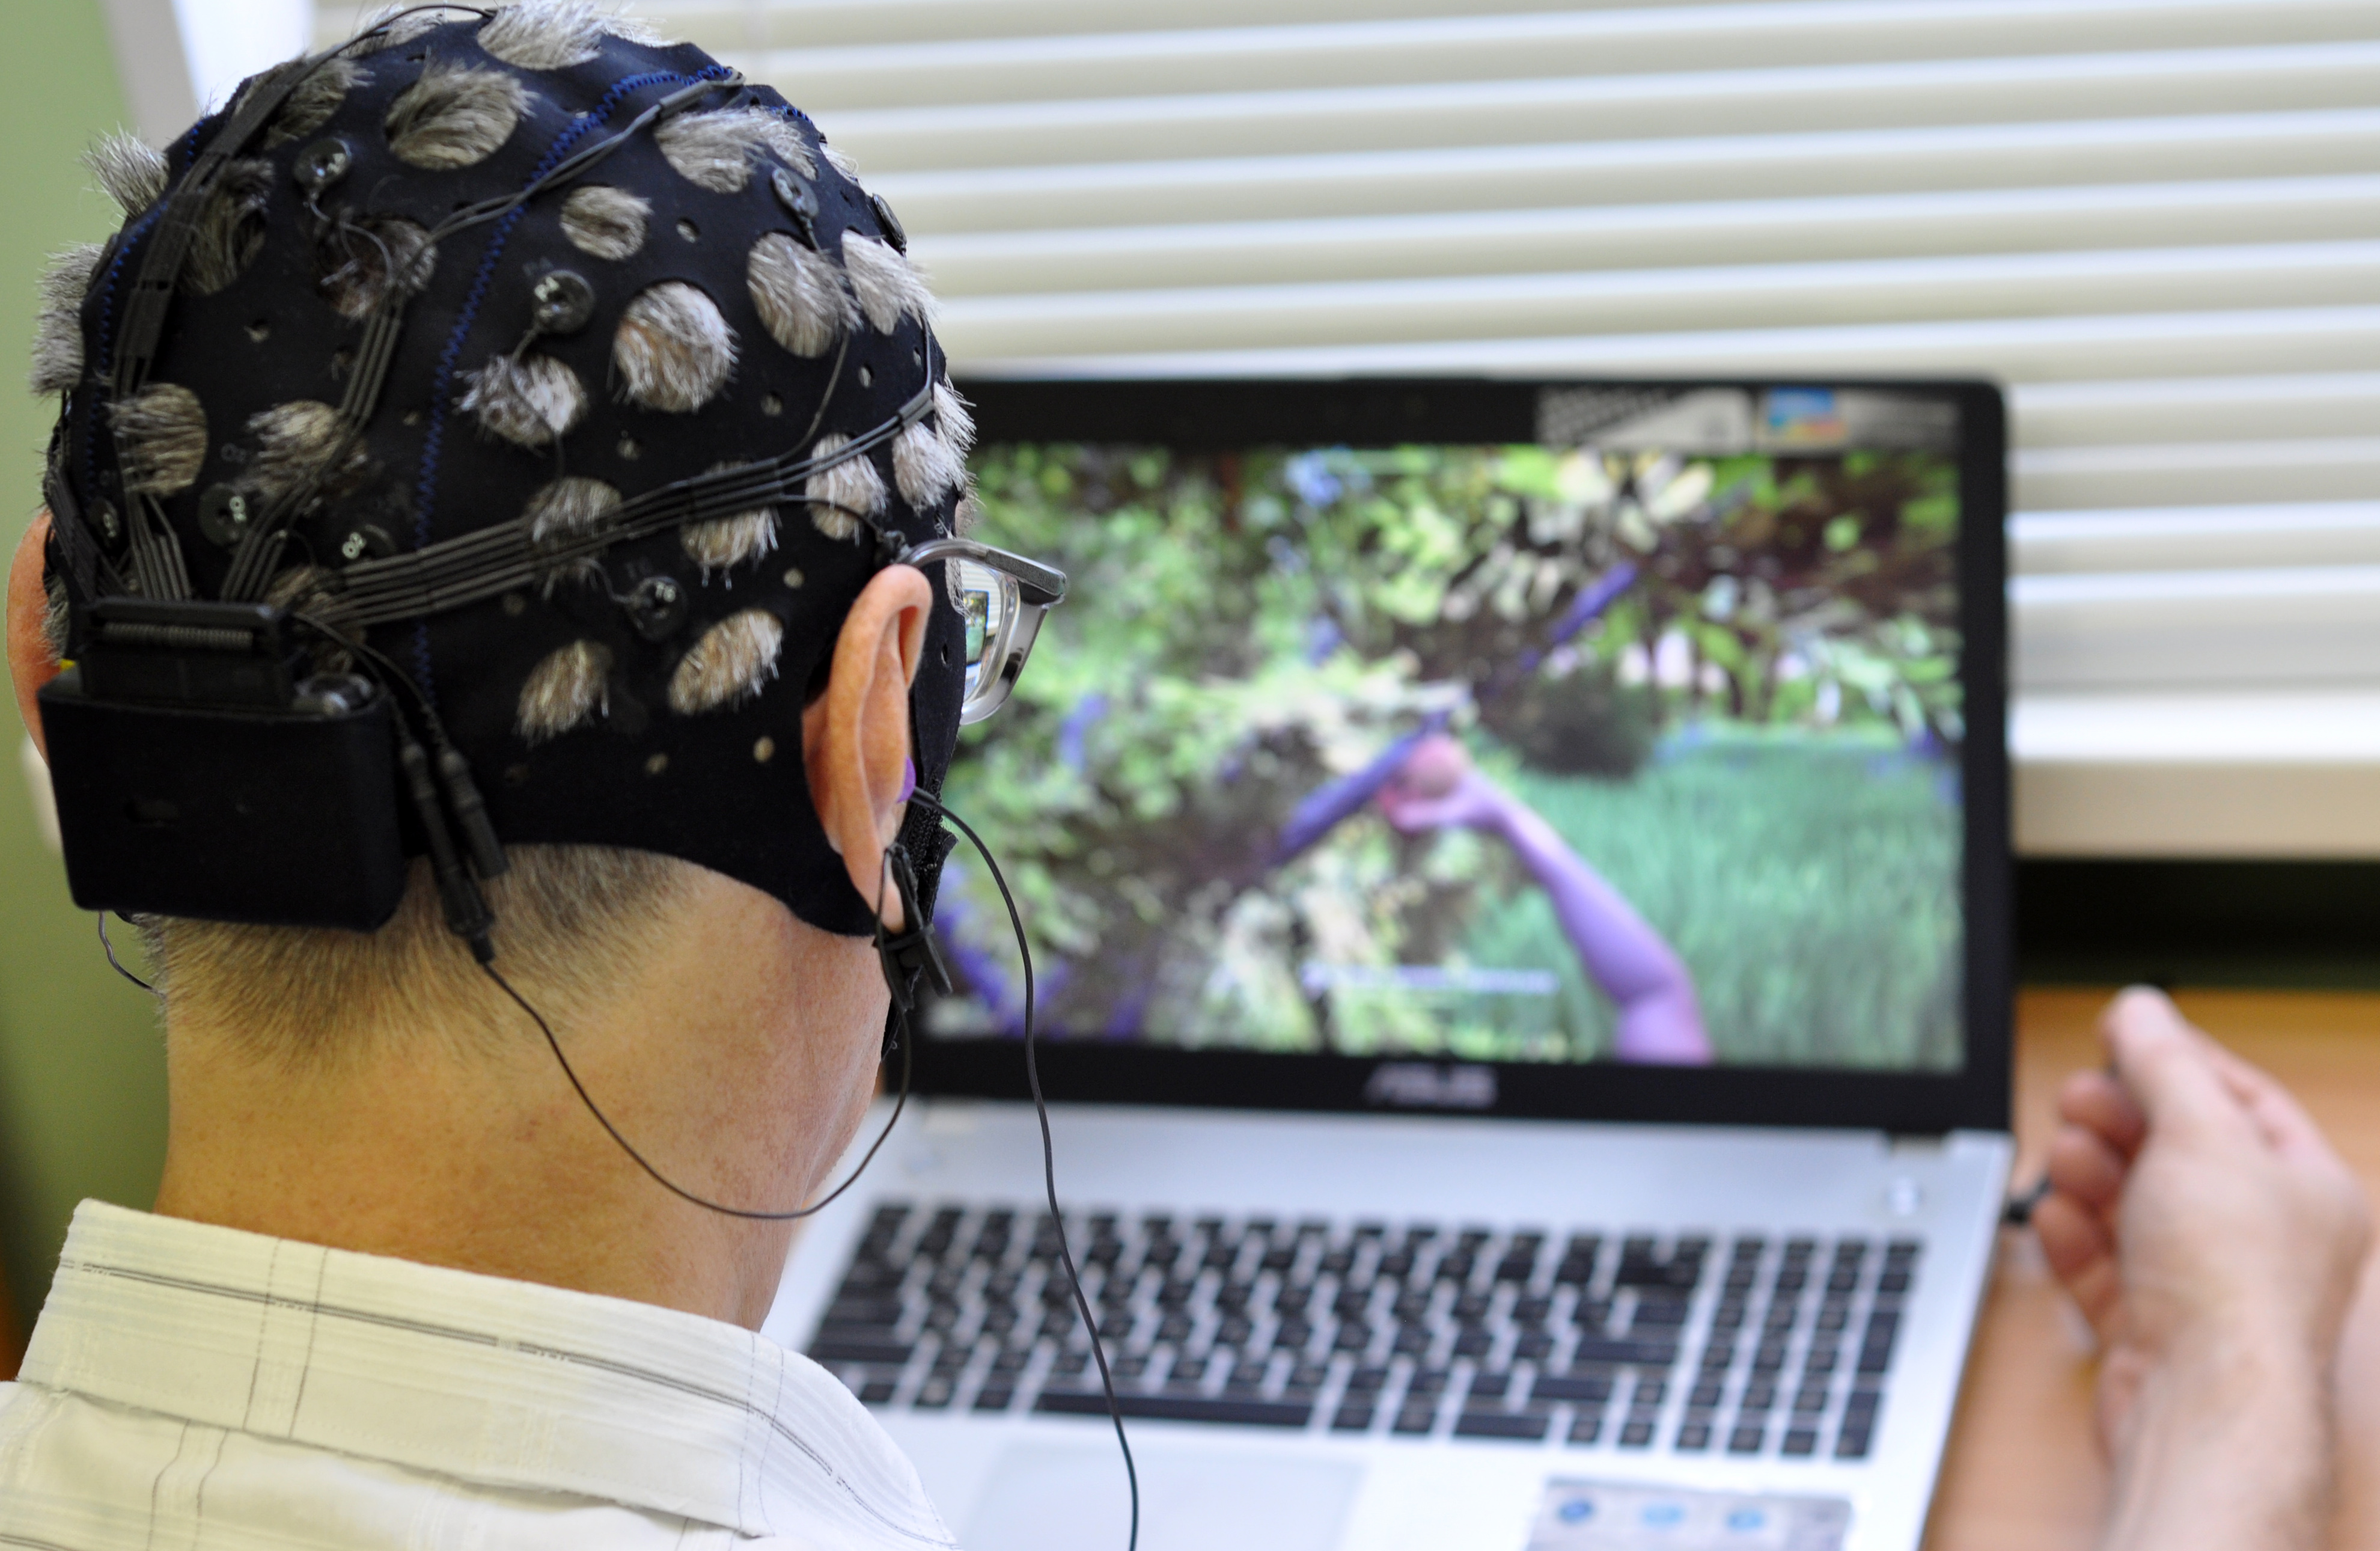
\includegraphics[width=\linewidth]{5.jpg}
    \end{minipage}
    \hfill 
    \begin{minipage}[h]{0.5\linewidth}
    \begin{itemize}
        \item Создание увлекательной игры.
        \item Увеличение эффективности реабилитационных процедур.
        \item Повысить стремление больных к выздоровлению.
    \end{itemize}
    \end{minipage}

\end{frame}
\section{Предлагаемое решение}

\begin{frame}
\frametitle{\insertsection} 
\framesubtitle{\insertsubsection}
\end{frame}
\section{Преимущества}

\begin{frame}
\frametitle{\insertsection} 
\framesubtitle{\insertsubsection}
    \begin{itemize}
        \item Высокий уровень кастомизации.
    \end{itemize}
\end{frame}


\section{Сроки и бюджет}

\begin{frame}
\frametitle{\insertsection} 
\framesubtitle{\insertsubsection}
\begin{itemize}
    \item Сроки: 2 месяца
    \item Бюджет: 500р.
\end{itemize}
\end{frame}


\section{Спасибо за внимание!}

\begin{frame}
\centering{\textbf{\Large Спасибо за внимание!}}
\end{frame}


\end{document}